\documentclass[twocolumn,amsmath,amssymb,floatfix,nature,shownopacs,footinbib,superscriptaddress]{revtex4-1} %linenumbers
\usepackage{amsmath,amssymb,natbib,bm,epsf,color}

\usepackage{hyperref}
%or \usepackage{url}
\usepackage{etoolbox}
\appto\UrlBreaks{\do\-}

\usepackage{graphicx}
\usepackage{color}
\usepackage[caption=false]{subfig}
\usepackage{booktabs} % for \toprule, \midrule, \bottomrule in tables

\newcommand{\rev}[1]{{\color{red} #1}}

\usepackage{soul}
\graphicspath{{/home/fbellisardi/code/topolity/paper/images/}}
\newcommand{\fixedDEMheight}{6cm}


\begin{document}

\title{Inferring Urban Morphology through Gravitational Work Minimization of Twitter-Derived Trajectories}

\author{Federico Bellisardi}\email{fbellisardi@ifisc.uib-csic.es}\affiliation{Instituto de F\'{\i}sica Interdisciplinar y Sistemas Complejos IFISC (CSIC-UIB), Campus UIB, 07122 Palma de Mallorca, Spain}

\author{Enrique Cano Su\"nen}
\affiliation{Universidad de Zaragoza, Spain}

\author{Ana Ruiz Varona}
\affiliation{Universidad San Jorge, Zaragoza, Spain}

\author{Jos\'e J. Ramasco}\email{jramasco@ifisc.uib-csic.es}
\affiliation{Instituto de F\'{\i}sica Interdisciplinar y Sistemas Complejos IFISC (CSIC-UIB), Campus UIB, 07122 Palma de Mallorca, Spain}

\maketitle

\textbf{Abstract}

\smallskip

\section*{Introduction}

\section*{Methods}
\subsection*{Twitter OD Data Reconstruction}

\label{sec:twitter-data}

% We based our analysis on geolocated Twitter data collected between 2015 and 2022 from more than fifty cities on every inhabited continent. Our aim was to convert these individual "check-ins" into coherent trajectories that reveal how people actually move through urban space. To achieve this, we extracted each tweet's spatial footprint - either a precise \texttt{POINT} coordinate (defined by a tuple of lat-lon coordinates) or a \texttt{POLYGON} bounding area (defined by 4 points vertices) - and reprojected all geometries into a single metric coordinate system, discarding any bounding polygons whose area exceeded 200 km$^2$. Timestamps were parsed and normalized to UTC, ensuring that every record was directly comparable regardless of local time zones or daylight-saving transitions. By reducing each tweet to its essential spatiotemporal components - where and when it occurred - we stripped away extraneous information and produce a lean, uniform dataset optimized for trajectory analysis. A representative sample of these processed records is shown in Table~\ref{tab:twitter-geometry-sample}.
% \begin{table}[ht]
%   \centering
%   \scriptsize
%   \setlength{\tabcolsep}{3pt}
%   \begin{tabular*}{\textwidth}{@{\extracolsep{\fill}} l l p{10cm} @{} }
%     \toprule
%     \textbf{Datetime} & \textbf{User} & \textbf{Geo-localization} \\
%     \midrule
%     2015-01-02 17:32:00 & \texttt{USER\_1} & \texttt{POINT (1.155948 41.087918)} \\
%     2015-01-05 10:05:20 & \texttt{USER\_2} & \texttt{POINT (2.156102 41.384112)} \\
%     2015-01-09 21:13:17 & \texttt{USER\_3} & \texttt{POINT (2.161144 41.391157)} \\
%     2015-01-15 10:00:55 & \texttt{USER\_4} & \texttt{POINT (2.186301 41.379876)} \\
%     2017-03-25 09:12:44 & \texttt{USER\_5} & \texttt{POLYGON ((12.625949 41.796313, 12.625949 41.852161, 12.704790 41.852161, 12.704790 41.796313, 12.625949 41.796313))} \\
%     2017-04-01 08:19:12 & \texttt{USER\_6} & \texttt{POLYGON ((13.282624 41.513575, 13.282624 41.618567, 13.381348 41.618567, 13.381348 41.513575, 13.282624 41.513575))} \\
%     \bottomrule
%   \end{tabular*}
%   \caption{Example records from the Twitter dataset, showing for each tweet the UTC timestamp, an anonymized user identifier, and its geospatial footprint—either as a precise POINT coordinate or as a POLYGON bounding area.}
%   \label{tab:twitter-geometry-sample}
% \end{table}

Next, we confronted the challenge of separating genuine human movement from automation, one-off events, and artifacts.  We begun by identifying accounts whose activity pace exceeded three posts per hour; such high-frequency behavior almost always reflects bots, live-event streams, or institutional feeds rather than individual movements.  Once those accounts were removed, we discarded any remaining users with fewer than three total posts, since a single hop or a pair of points cannot trace a meaningful path.  Finally, even plausible streams could hide implausible leaps: we computed, for each consecutive pair of posts, the straight-line distance in meters and the elapsed time in hours, derive an implied velocity, and eliminate any segments exceeding 900 km/h: this approach filtered out multi-account profiles—often corporate or organizational actors—ensuring our analysis focused solely on individual users. 

This three-stage cleansing leaft us with a curated collection of trajectories that credibly represent human mobility. 
% Figure~\ref{fig:rej_uids_by_reason} illustrates the percentage of rejected user identified by rejection reason across four representative cities, with colors denoting categories: pink for fewer than three tweets, blue for suspected bot activity, and green for excessive speed.

% \begin{figure}[!htbp]
%   \centering
%   \begin{subfigure}[b]{0.45\textwidth}
%     \centering
%     
\includegraphics[width=0.8\linewidth]{rejected/rejected_uids_by_reason_pie_madrid.png}
%     \caption{Madrid, Spain (286\,760 UIDs)}
%     \label{fig:rej_madrid}
%   \end{subfigure}
%   \hfill
%   \begin{subfigure}[b]{0.45\textwidth}
%     \centering
%     
\includegraphics[width=0.8\linewidth]{rejected/rejected_uids_by_reason_pie_mexico.png}
%     \caption{Mexico City, Mexico (420\,898 UIDs)}
%     \label{fig:rej_mexico}
%   \end{subfigure}

%   \vspace{1em}

%   \begin{subfigure}[b]{0.45\textwidth}
%     \centering
%     
\includegraphics[width=0.8\linewidth]{rejected/rejected_uids_by_reason_pie_paris.png}
%     \caption{Paris, France (552\,465 UIDs)}
%     \label{fig:rej_paris}
%   \end{subfigure}
%   \hfill
%   \begin{subfigure}[b]{0.45\textwidth}
%     \centering
%     
\includegraphics[width=0.8\linewidth]{rejected/rejected_uids_by_reason_pie_saopaulo.png}
%     \caption{Sao Paolo, Brazil (428\,885 UIDs)}
%     \label{fig:rej_saopaolo}
%   \end{subfigure}

%   \caption{Percentage of UIDs rejected for each reason, expressed as a proportion of the total UIDs removed in each selected city (showing the total number of users removed from each city).  
%     Colors denote categories: \emph{pink} = less than 3 tweets in 8 years; \emph{blue} = suspected bot activity; \emph{green} = excessive speed.}
%   \label{fig:rej_uids_by_reason}
% \end{figure}

Having distilled the data to its essence, we superimposed a regular, square grids—of side length 1000 m—over the projected extent of each city. Then we computed the overall bounding box of the reprojected tweets and subdivided it into integer-indexed cells, yielding a uniform lattice that simplifies both analysis and interpretation. An efficient spatial index then assigned each tweet to its corresponding cell with the following logic: precise POINT geometries mapped directly via integer division, while POLYGON footprints were first intersected with the grid and then resolved—by selecting the cell of maximum overlap. In this way, every tweet had been endowed with a unique cell identifier and an associated confidence score, enabling consistent, multiscale trajectory analysis.  

\begin{figure*}[t!]
\centering
\subfloat[\textbf{Working days }]{
    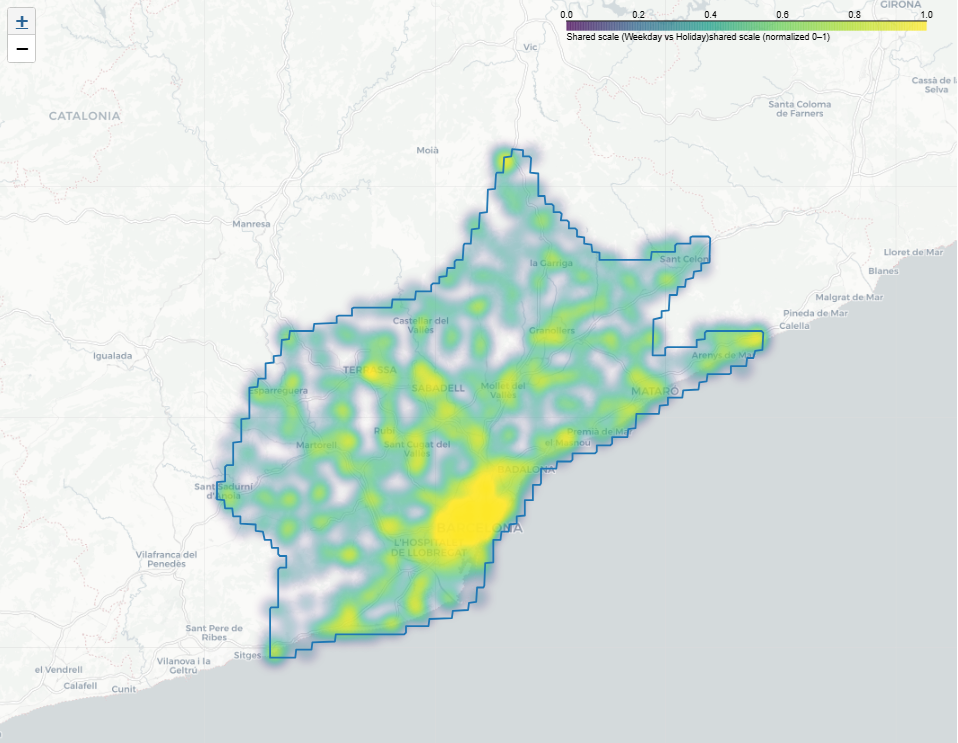
\includegraphics[width=0.48\textwidth]{images/bcn_heatmap_wd.png}
    \label{fig:heatmap_wd}
}
\hfill
\subfloat[\textbf{Holidays}]{
    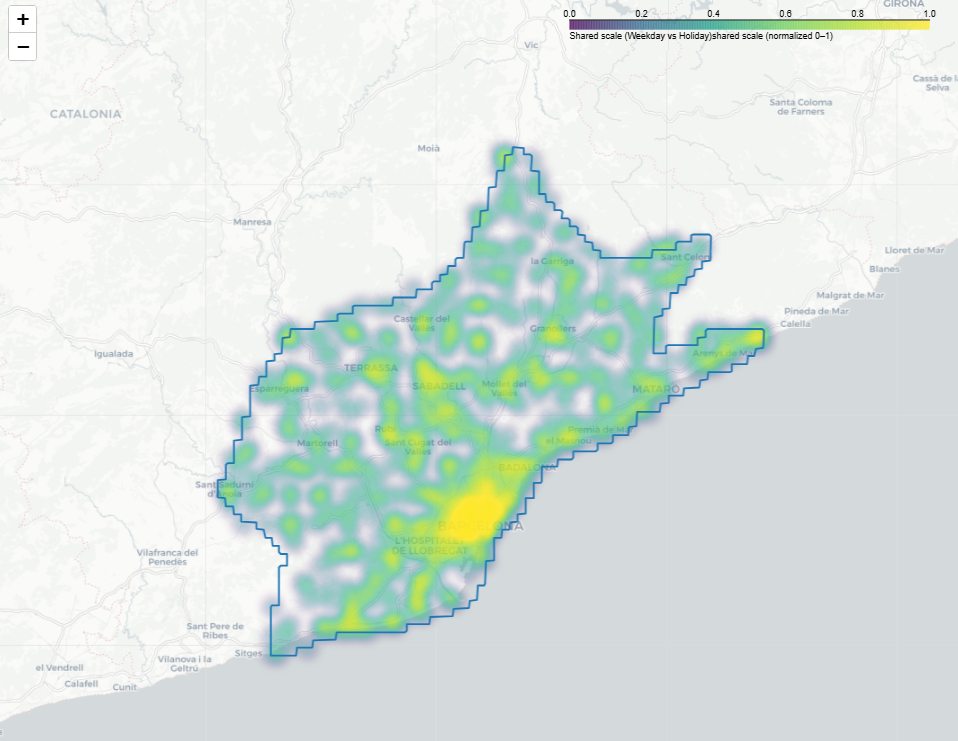
\includegraphics[width=0.48\textwidth]{images/bcn_heatmap_hd.png}
    \label{fig:heatmap_hd}
}
\caption{\textbf{Origin-destination flow heatmaps for Barcelona.}
\textbf{a–b}, Working days (\textbf{a}) and holidays (\textbf{b}) OD flow heatmaps, illustrating the spatial distribution of user movements across the city. The color intensity of each cell corresponds to the normalized number of transitions between origin-destination pairs, with a color bar indicating the scale. The axes represent the grid cell indices along the x and y directions, respectively.}
\label{fig:flow_heatmap}
\end{figure*}

The final transformation converted these cell-tagged trajectories into origin-destination flows.  We label each date as a working day or holiday—either by consulting a calendar API—and then, for each user, chronologically sequence their visited cells.  Every successive pair of cells contributed one unit to the corresponding entry in an OD matrix.  Summing over all users and days of the same type yielded two comprehensive flow tables—one for workdays and one for holidays—where each row specified an origin cell, a destination cell, and the total count of observed transitions.  These OD matrices form the empirical backbone of our gravitational-work minimization, enabling us to probe how subtle perturbations to the urban fabric—through translations, rotations, or scalings—reshape the uphill effort embedded in real human journeys. In Figure \ref{fig:flow_heatmap} we show an example of the OD matrix flows reconstructucted for the city of Barcelona for the working days (left panel a) and holidays (right panel b).


\subsection*{Study Areas and City Boundaries}
\label{sec:city-boundaries}

\begin{figure*}[t!]
\centering
\setlength{\tabcolsep}{0pt}

\newlength{\FIGH}\setlength{\FIGH}{0.40\textheight}
\newlength{\ROWSEP}\setlength{\ROWSEP}{1.2ex}
\newlength{\RONE}\setlength{\RONE}{0.34\FIGH}
\newlength{\RTWO}\setlength{\RTWO}{0.34\FIGH}
\newlength{\RTHR}\setlength{\RTHR}{0.34\FIGH}

\begin{minipage}[t]{0.30\textwidth}
  \vspace{0pt}
  \subfloat[\textbf{Overview}\label{fig:overview}]{
    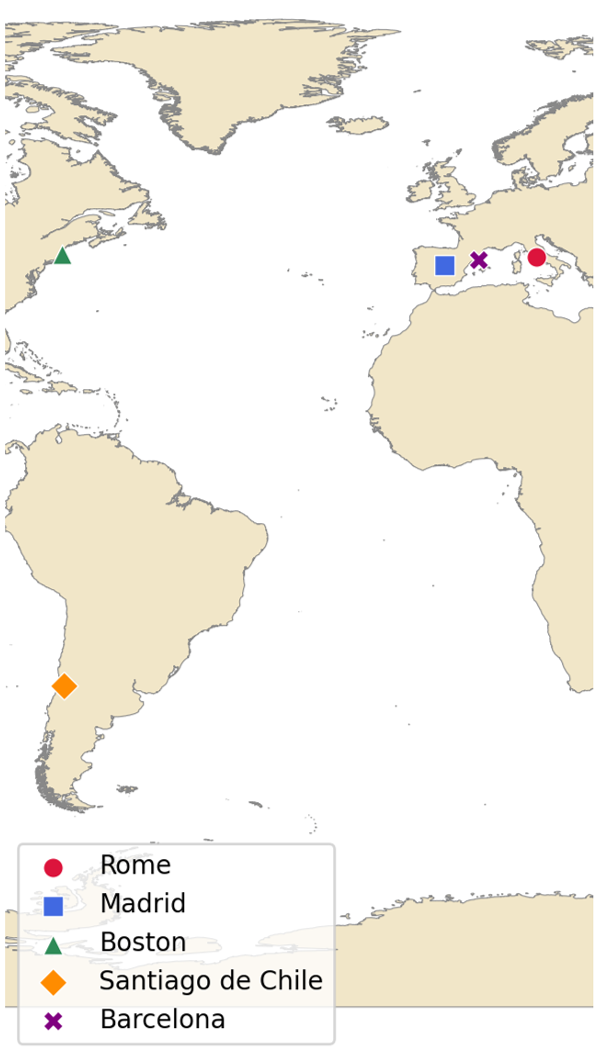
\includegraphics[height=\FIGH]{images/cities.png}
  }
\end{minipage}%
\hfill
\begin{minipage}[t]{0.70\textwidth}
  \vspace{0pt}

  \subfloat[\textbf{Rome}\label{fig:rome}]{
    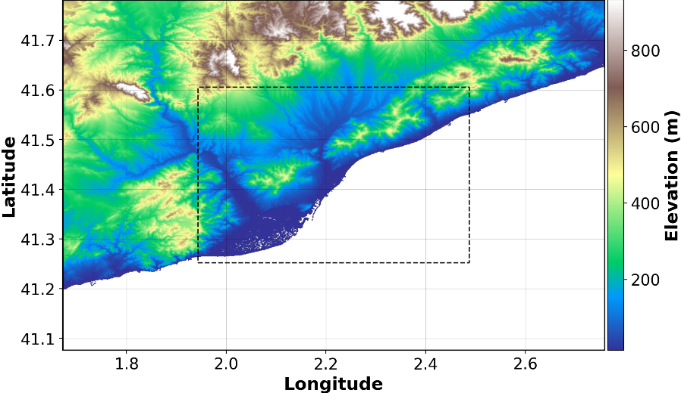
\includegraphics[height=\RONE]{images/dem/rome_dem.png}
  }\hfill
  \subfloat[\textbf{Madrid}\label{fig:madrid}]{
    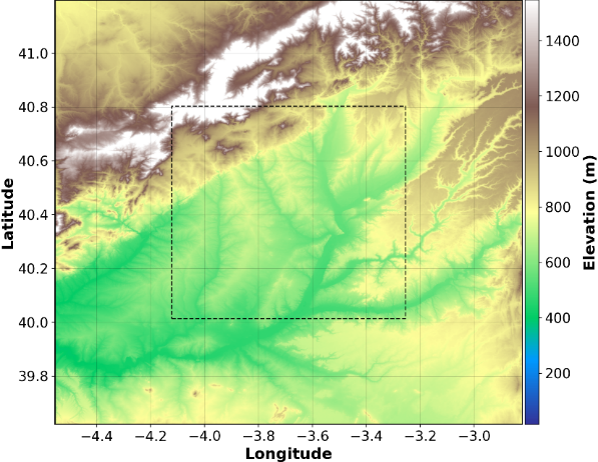
\includegraphics[height=\RONE]{images/dem/madrid_dem.png}
  }\\[\ROWSEP]

  \centering
  \subfloat[\textbf{Boston}\label{fig:boston}]{
    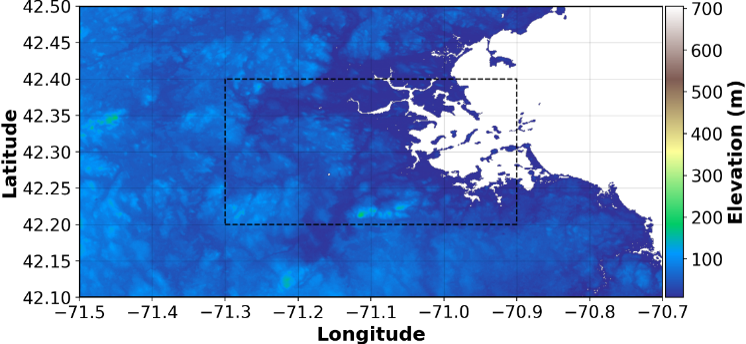
\includegraphics[height=\RTWO]{images/dem/boston_dem.png}
  }\\[\ROWSEP]

  \noindent
  \subfloat[\textbf{(e) Santiago}\label{fig:santiago}]{
    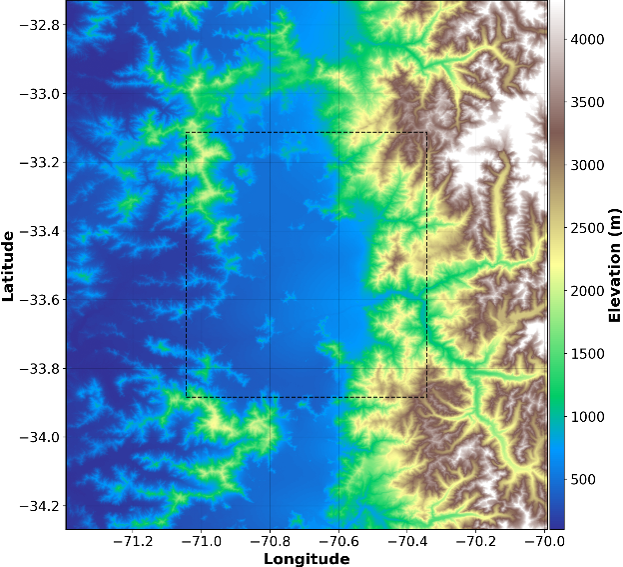
\includegraphics[height=\RTHR, width=5cm]{images/dem/santiago_dem.png}
  }\hfill
  \subfloat[\textbf{(f) Barcelona}\label{fig:barcelona}]{
    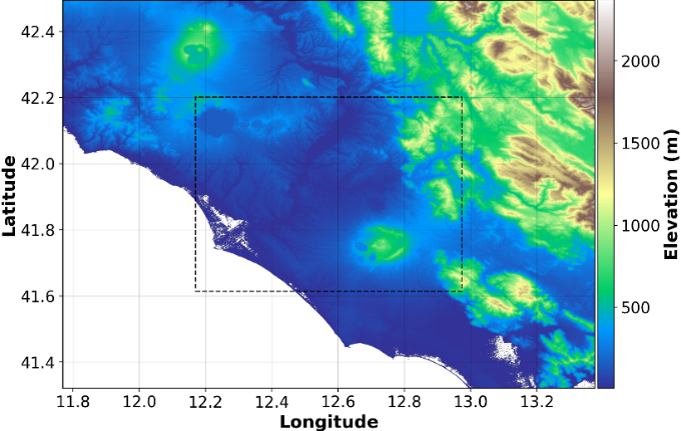
\includegraphics[height=\RTHR]{images/dem/barcelona_dem.png}
  }

\end{minipage}

\caption{\textbf{Topography of selected cities.}
Global overview on the left (\textbf{a}); local maps on the right in a 2+1+2 layout (\textbf{b–f}).}
\label{fig:city_map}
\end{figure*}


For this study, we selected a set of cities that represent different urban landscapes and mobility patterns. The cities included in our analysis are shown in Figure~\ref{fig:city_map} and include Rome (Italy), Madrid (Spain), Barcelona (Spain), Boston (USA) and Santiago del Chile (Chile)..




The geographic boundaries of each city were defined using the spatial dataset delineates the boundaries of Functional Urban Areas (FUA) of Urban Centres , which was obtained from the European Commission's Joint Research Centre (JRC) \cite{jrc-fua}. This dataset provides a comprehensive and standardized definition of urban areas across Europe and beyond, allowing for consistent comparisons of urban morphology and mobility patterns. In the Supplementary Material (see Appendix \ref{sec:city-characteristics}), we provide a table summarizing the key characteristics of each city, including population size, area, and the number of Twitter-derived trajectories analyzed. Moreover, we show the boundaries of the FUA for each city in Figure~\ref{fig:fua_boundaries}, which illustrates the spatial extent of the area as defined by the FUA dataset. Each figure represents the functional connections between the urban core and surrounding areas, which are crucial for understanding urban morphology and mobility patterns.

The FUA boundaries were used to extract the relevant urban network data from OpenStreetMap (OSM) and to define the spatial extent for the analysis of Twitter-derived trajectories. The FUA boundaries were reprojected to match the coordinate system of the Twitter-derived trajectories, ensuring that all spatial operations were consistent.



\subsection*{Gravitational Work Computation}
% Define work minimization, edge sampling, and uphill work aggregation.
To quantify the topographic cost of movement, we first acquired a high-resolution SRTM digital elevation model (DEM) for each city, as described in Sec. %\ref{sec:elevation-data}.

At this point, we discretized each road-segment into evenly spaced sample points at a fixed interval $\Delta s = 10\,$m.  For a given edge $e$, of the graph $G$, of total length $L_e$, we set the total number of elevation-sampling points placed along edge $e$ as
\[
    N_e \;=\;\Bigl\lceil \frac{L_e}{\Delta s}\Bigr\rceil + 1,
    \]
    and defined the sampling distances
    \[
    s_i \;=\;\frac{i}{N_e - 1}\,L_e,
    \quad i = 0,1,\dots,N_e-1.
\]
Each point $\mathbf{x}_i$ was obtained by interpolating the linestring geometry of $e$ at distance $s_i$, then projected to geographic coordinates via the DEM's affine transform.  We queryed the DEM at $\mathbf{x}_i$ (using rasterio's sampling routine) to retrieve an elevation value $z_i$.  The resulting elevation profile for edge $e$ is therefore the ordered sequence
\[
\bigl\{(\mathbf{x}_i, z_i)\bigr\}_{i=0}^{N_e-1},
\]
which provided the detailed vertical trace needed for accurate uphill-work computations. 












\subsection*{Copresence dynamic network}

A first question to address is 

\begin{figure}
%\includegraphics[width=\columnwidth]{Fig1_v4.pdf}
\caption{\textbf{London Heathrow Airport aggregated copresence network of one month data. a} Sketch ... .}\label{fig1}
%RG: 2DO: panel C and D are too small to be read
\end{figure}



 
\subsection*{EBlablaba}

The contact network is 

\begin{table}[h!]
\begin{center}
\begin{tabular}{l*{3}{c}r}
Name            & Explanation  &    Reference \\
\hline
SIR               &   Original SIR   &  \cite{mkhatshwa2010modeling} \\
SEIR             &    SEIR for H1N1     & \cite{balcan2009seasonal} \\
EBOLA               &   SEIR for EBOLA    &  \cite{gomes2014} \\
SARS-Cov2:   &     SEIIR for SARS-Cov2     & \cite{2020didomenico} \\
SIRR3               &   SIR double infectivity   &  \cite{mkhatshwa2010modeling} \\
SIR30               &   SIR with 30' time scale & \cite{mkhatshwa2010modeling} \\
\end{tabular}
\caption{List of abbreviation for the epidemic models here considered and respective reference to the literature for the choice of the epidemic parameters.}
\label{table:models}
\end{center}
\end{table}

\subsection*{Spatial Immunization}

The diseases mentioned


\section*{Results}

\subsection*{Simplest model: SIR}

\begin{figure}
%\includegraphics[width=\columnwidth]{Fig2_v3.pdf}
\caption{\textbf{Risk of contagion in space.} Cells in the airport area with a heatmap showing the fraction of contagions occurring in them when running the SIR model. In \textbf{a}, after one day of simulation and in \textbf{b} after two days. }\label{sirspac}
\end{figure}  

We start by studying the simplest epidemic model: the SIR, with only susceptible, ...

\subsection*{SEIR family}


%\begin{figure}
%\includegraphics[width=\columnwidth]{heatsupp/figbohseir.pdf}
%\caption{\textbf{UV surface irradiation effect for SEIR. a} Outbreak probability per each value of irradiated surface. \textbf{b} Infections frequency per time slot. Per each time slot we count how many infections occurred. \textbf{c} Destinations affected. $N_i/N_0$ represents the relative infections over the UV-free infections per each destination. This plot depicts how fast a destination lowers its infected population by increasing the UV irradiated surface. \textbf{d} Infection targets composition. $I_i/I_0$ represents the average percentage of destinations composing the overall infections per each value of irradiated surface.}\label{seirout}
%\end{figure}




\section*{Discussion and conclusions}


In this work, we have shown how using a network approach it is possible to reduce the complexity of the spatial trajectory in Heathrow airport and encode them in a temporal network of copresences among different categories of users. Based on those networks, we run four different compartmental models from the literature to mimic the spreading of four different strains, namely SARS, H1N1, EBOLA and SARS-Cov2, each one with different epidemic parameters. From these simulations we are able to detect workers as the most exposed and infectious category of individuals inside the airport, independently of the virus under study. This is due to the fact that employees are the agents more often infected: they recurrently appear in the airport day after day and they come in contact with many passengers, but also colleagues, whereas passengers generally cross the area of the airport only for few hours before departure or after arrival. To fully describe the movements across the airport, we had to supersample the trajectories creating a standard day which is of course only an approximation of reality, but still these different behaviors hold true in our simulations. Second in the rank by infectiousness we find connecting passengers, since they are the travelers who spend more time inside the airport waiting for connections between a flight and the next. Restaurants, bars and in general relax areas are the places where most of the copresences (and contagions) happen and this is where indeed connecting travelers use to rest and stop for a long time waiting and interacting with employees. 

By applying a policy of spatial immunization based on non-harmful UV lights or similar spatial immunization methods such as frequent cleaning and disinfection of surfaces, air filters, ozone, etc, to hygenize the area of terminals, we are able to decrease the effect of infectious droplets, aerosols and contaminated air or surfaces. By selecting the places to immunize and their number using infection hotspots as predicted by the models, it is possible to sensibly decrease the contagion probability and the intensity of outbreaks for every disease studied. In all of them there is a common attribute and it is that the characteristic times of the disease evolution, e.g., latency period, are longer than the period spent by most of the users in the airport. This makes possible that the simplest SIR model, in which only contagion events are relevant, is enough to produce an accurate estimation of the contagion hotspots valid for most diseases. Note that these hotspots are not only characterized by the concentration of people but by a balance between time spent and individual concentration: places as cafeterias, access points, etc, are the most critical hotspots to immunize. Still, the method is general and in the eventuality of considering a quick evolving disease the hotspots should be recalculated with an \textit{ad hoc} model.   

We include an analysis further disaggregating the average probability of traveling from each terminal of Heathrow to UK, European and Intercontinental destinations around the world. Thanks to this detailed information, we are able to estimate the average threat represented by the development of an outbreak in the airport for these three classes of destinations for any of the four types of virus. Our spatial immunization policy helps containing the menace of passengers getting infected in the terminals while traveling to other destinations, potentially delaying the massive seeding of new infected individuals from London to the rest of the world. Unfortunately, this policy seems to be less effective on workers, who exhibit a longer exposure to the virus with respect to passengers. This suggests that targeted vaccinations on the airport employees may further reduce the probability and even the severity of an outbreak within every strain scenario. However, when vaccination is not available, in all the cases we register an important decrease on the outbreak probability and on the total amount of infected among all the destinations and all the categories of individuals. This same approach finds immediate direct applications of a similar spatial immunization technique to many other buildings like hospitals, schools, universities, train stations and museums, potentially reducing the appearance of new and uncontrolled outbreaks even in the absence of vaccines. All these places share the common feature of having a large in and outflow of visitors and by a set of workers that appear in some areas of the infrastructure recurrently. This leads to strong heterogeneities in the location and duration of the contacts among visitors and between visitors and workers, which allows us to define a successful spatial immunization strategy based on a hospot analysis. 



\section*{Data Availability Statement}

Mobility data is available from Cuebiq through their Data for Good program (\url{https://www.cuebiq.com/about/data-for-good/}). Restrictions apply to the availability of this data, which was used under license for the current study.

\section*{Acknowledgements}

M.M. acknowledges financial support of ... J.J.R. acknowledge funding from the project ...

\section*{Author Contribution}
To decide

\bibliographystyle{nature.bst}

\bibliography{references.bib}

\end{document}

%*****************************************
%*****************************************
%*****************************************
%*****************************************
%***************************************** 


%***************************__

